\documentclass{standalone}
\usepackage{amsmath,amssymb,amsthm}
\usepackage{tikz}
\usetikzlibrary{decorations.markings}
\usetikzlibrary{arrows,automata}
\usetikzlibrary{positioning}
\usetikzlibrary{arrows.meta,positioning}

\begin{document}
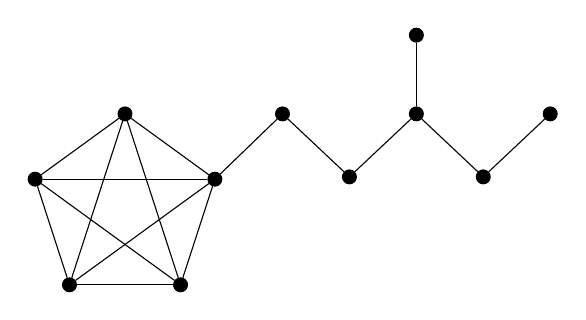
\begin{tikzpicture}[
    mycircle/.style={
        circle,
        draw=black,
        fill=black,
        fill opacity = 1,
        inner sep=0pt,
        minimum size=5pt,
        font=\small},
    nocircle/.style={
        circle,
        draw=black,
        fill=black,
        fill opacity = 1,
        inner sep=0pt,
        minimum size=0.45pt,
        font=\small},
    myarrow/.style={-},
    dottedarrow/.style={-,dashed},
    thiccarrow/.style={-,line width=0.9pt},
    node distance=1.2cm and 1.5cm
]

\begin{scope}
    \begin{scope}[rotate=90]
        \foreach \x/\y in {0/0,72/1,144/2, 216/3, 288/4}{ % color in outer layer
        \node[mycircle] (\y) at (canvas polar cs: radius=1.2cm,angle=\x){};
        }
    \end{scope}

    \path[every node/.style={font=\sffamily\small}]
        (0) edge [color=black] (1)
        (0) edge [color=black] (2)
        (0) edge [color=black] (3)
        (0) edge [color=black] (4)
        (1) edge [color=black] (2)
        (1) edge [color=black] (3)
        (1) edge [color=black] (4)
        (2) edge [color=black] (3)
        (2) edge [color=black] (4)
        (3) edge [color=black] (4);

    \node[mycircle] (a) at (2, 1.2) {};
    \node[mycircle] (b) at (2.85, 0.4) {};
    \node[mycircle] (c) at (3.7, 1.2) {};
    \node[mycircle] (d) at (4.55, 0.4) {};
    \node[mycircle] (e) at (5.4, 1.2) {};

    \path[every node/.style={font=\sffamily\small}]
        (4) edge [color=black] (a)
        (a) edge [color=black] (b)
        (b) edge [color=black] (c)
        (c) edge [color=black] (d)
        (d) edge [color=black] (e);

    \node[mycircle] (x) at (3.7, 2.2) {};

    \path[every node/.style={font=\sffamily\small}]
        (x) edge [color=black] (c);
\end{scope}
\end{tikzpicture}
\end{document}